
\documentclass[11pt]{article}

\usepackage[latin1]{inputenc}
\usepackage{amssymb}
\usepackage{amsmath}
\usepackage{amscd}
\usepackage{amsthm}
\usepackage{amsfonts}
\usepackage{enumerate}
\usepackage{graphicx}
\usepackage{url}
\usepackage[breaklinks=true,hyperref]{hyperref}
\usepackage{amssymb}
\usepackage[dvips]{color}
\usepackage{epsfig}
\usepackage{mathrsfs}
\usepackage{comment}


\pdfpagewidth 8.5in
\pdfpageheight 11in
\topmargin -1in
\headheight 0in
\headsep 0in
\textheight 8.5in
\textwidth 6.5in
\oddsidemargin 0in
\evensidemargin 0in
\headheight 75pt
\headsep 0in
\footskip .75in


\newenvironment{ee}{\begin{enumerate}}{\end{enumerate}}
\newenvironment{ii}{\begin{itemize}}{\end{itemize}}

\newcommand{\argmax}{\arg\!\max}
\newcommand{\argmin}{\arg\!\min}

\newcommand{\abs}[1]{\left\vert #1 \right\vert}
\newcommand{\Var}{\text{Var}}
\newcommand{\Cov}{\text{Cov}}
\renewcommand{\Pr}[2]{\mathop{\text{Pr}}_{#1} \left[ #2 \right]}

\def\RR{\mathbb R}
\def\CC{\mathbb C}
\def\QQ{\mathbb Q}
\def\ZZ{\mathbb Z}
\def\NN{\mathbb N}
\def\powset{\mathbb P}
\def\FF{\mathbb F}

\def\e{\epsilon}
\def\d{\delta}
\def\p{\partial}
\def\Chi{\chi}

\def\ds{\displaystyle}
\newcommand{\vs}[1]{\vspace{#1 pt}}

\def\tensor{\otimes}
\def\xor{\oplus}

\newcommand{\floor}[1]{\left\lfloor #1 \right\rfloor}
\newcommand{\ceil}[1]{\left\lceil #1 \right\rceil}
\newcommand{\field}[1]{\mathbb #1}
\newcommand{\inner}[2]{\langle #1,#2\, \rangle}
\newcommand{\norm}[2]{\| #1 \|_{#2}}
\newcommand{\ket}[1]{| #1 \rangle}
\newcommand{\bra}[1]{\langle #1 |}
\newcommand{\dirac}[2]{\langle #1 | #2\, \rangle}


\newcommand{\bracket}[1]{\langle #1 \rangle}
\newcommand{\paren}[1]{\left( #1 \right)}
\newcommand{\set}[1]{\left\{ #1 \right\}}

\newcommand{\bset}{\left\{0,1\right\}}

\newcommand{\inv}{^{-1}}
\newcommand{\til}{\widetilde}
\newcommand{\sign}{\mathrm{sgn}\;}
\renewcommand{\mod}{\text{ mod }}

\newcommand{\poly}{\text{poly}}
\newcommand{\polylog}{\text{polylog}}
\newcommand{\tsc}[1]{\textsc{#1}}
\newcommand{\tmc}[1]{\mathcal{#1}}

\newcommand{\Co}{{\sf Co-}}
\newcommand{\co}{{\sf co}}
\newcommand{\modpoly}{/ \text{poly}}
\newcommand{\SPACE}{{\sf SPACE}}
\newcommand{\TIME}{{\sf TIME}}
\def\D{{\sf D}}
\def\N{{\sf N}}
\def\P{{\sf P}}
\def\L{{\sf L}}
\def\E{{\sf E}}
\newcommand{\promise}{\textsf{promise}}

\newcommand{\NP}{{\sf NP}}
\newcommand{\PSPACE}{{\sf PSPACE}}
\newcommand{\EXP}{{\sf EXP}}

\newcommand{\BP}{{\sf BP}}

\newcommand{\NL}{{\sf NL}}

\newcommand{\NC}{{\sf NC}}
\newcommand{\AC}{{\sf AC}}
\newcommand{\RP}{{\sf RP}}
\newcommand{\BPP}{{\sf BPP}}
\newcommand{\PH}{{\sf PH}}
\newcommand{\PP}{{\sf PP}}
\newcommand{\IP}{{\sf IP}}
\newcommand{\AM}{{\sf AM}}
\newcommand{\MA}{{\sf MA}}
\newcommand{\PCP}{{\sf PCP}}

\newcommand{\FO}{{\sf PA}}
\newcommand{\SO}{{\sf PA}}
\newcommand{\PA}{{\sf PA}}
\newcommand{\ZF}{{\sf ZF}}
\newcommand{\ZFC}{{\sf ZFC}}

\newtheorem{theorem}{Theorem}[section]
\newtheorem{lemma}[theorem]{Lemma}
\newtheorem{proposition}[theorem]{Proposition}
\newtheorem{prop}[theorem]{Proposition}
\newtheorem{corollary}[theorem]{Corollary}
\newtheorem{conjecture}[theorem]{Conjecture}

%\theoremstyle{definition}
\newtheorem{example}[theorem]{Example}
\newtheorem{problem}[theorem]{Problem}
\newtheorem{definition}[theorem]{Definition}
\newtheorem{question}[theorem]{Question}
%\theoremstyle{remark}

\newtheorem{remark}[theorem]{Remark}
\numberwithin{equation}{section}

\renewcommand{\theequation}{\thesection.\arabic{equation}}




\begin{document}

\title{{\bf Efficient Inference in Probabilistic Computing} \\ M.Eng Propsal}
\author{Jeff Wu}
%\address{}
%\email{}
\date{}
\maketitle
%
%\begin{center} \begin{LARGE} {\sc \bf Title} \vs{6}

%{\sc M.Eng Proposal} \vs{9}

%\end{LARGE} { \Large \textsc{Jeff Wu}}

%\end{center}

\begin{abstract}
\end{abstract}

\section{Introduction}

Probabilistic programming languages are generalizations of programming languages, in which procedures are replaced with random procedures that induce distributions.  Probabilistic computing thus allows for easy description and manipulation of probability distributions, letting one describe classical AI models in compact ways.  

A core operation of probabilistic programming languages is inference, which is, in general, a difficult computational problem \cite{?}.  However, Markov chain Monte Carlo (MCMC) methods converge quite quickly to the posterior distribution for a large class of inference problems.  Much effort has been devoted to studying in which cases this inference is efficient, and how to make it so.  

% introduction: restate goals from above, of course including which research direction (parallelism; noise variables; connections to deterministic algorithms like sorting) we actually did


%INTRO
%build pcp engine which i understand well
%tested on variety of problems
%study tractability of inference on other harder problems
%do performance engineering / parallelism

%write-up spec of language
%write-up test cases

%write mixture-model

%\subsection{Outline}

%In this paper, we first give an overview of our language and its implementation.  



\section{Language description}

\subsection{Values}

A {\bf value} is a valid binding for a variable, in our language.  For example, integers, floats, and booleans are valid values.  We call these primitive values.  Another type of value is a {\bf procedure}, a function which gets applied to arguments and returns (not necessarily primitive) values.  

These procedures should be non-deterministic.  To allow for this, we can imagine that there is a special procedure, call it {\tt bernoulli}, which takes an argument $p$, and outputs 0 or 1, with probabilities $1-p$ and $p$, respectively.  Arbitrary random procedures can then be built up using this one.   We will see later that we actually can and will allow for something far more general than random procedures.

%Suppose I declare in some program that {\tt x} is determined by a coin flip.  But on any given execution of the program, {\tt x} must take on one of two values.  \vspace{6 pt}


\subsection{Expressions and Environments}

{\bf Expressions} are syntactic building blocks, which specified as being one of the following:
\begin{itemize}
\item Atomic expressions:
\begin{itemize}
\item A value itself.
\item A variable name.
\end{itemize}
\item Non-atomic expressions
\begin{itemize}
\item An application of an expression to a list of argument expressions.
\item A function, consisting of some variable arguments, and a body expression.
\item An if statement, consisting of a branching expression, and two child expressions.
\item An operator statement, consisting of an operator (e.g. == , $<$ , + , $\times$ , {\tt AND}, {\tt OR}, {\tt NOT}) and a list of argument expressions.
% \item A switch statement, consisting of a branching expression, and a list of child expressions
\end{itemize}
\end{itemize}

Expressions are {\bf evaluated}, so that they take on some value.  Their evaluation is relative to an {\bf environment}, in which variable names may be bound to values.  

Evaluation happens recursively.  If an invalid expression is ever given (e.g. the first expression in an application isn't a procedure, or we call the equality operator with three arguments), an error is thrown.  

\subsection{Directives}

There are four primitive operations, called {\bf directives}, which the language supports.  They are:

\begin{enumerate}
\item {\tt sample(expr)} : 

Evaluates with respect to the global environment to sample a value for the expression {\tt expr}.

\item {\tt assume(name, expr)} : 

Samples a value for the expression {\tt expr}, and then binds {\tt name}, a string variable name, to the resulting value in the global environment.

\item {\tt observe(expr, val)} : 

Observes the expression {\tt expr} to have been evaluated to the value {\tt val}.

\item {\tt infer()} : 

Runs a single step of the Markov Chain.  

\end{enumerate}

The result of calling {\tt infer()} sufficiently many times, should be that sampling gives the posterior distribution for expressions, conditioned on all the observed values.  
%The {\tt observe} primitive is required to be 

\section{Inference}

Inference is by far the most complicated of the directives, and also the most important.  Performing inference is the reason we are interested in probabilistic programming languages in the first place.  

% if we observe(blah, true), observe(blah, false)

%    - language definition with examples
%                - XRPs: what they are, and how to add them


%
%        - test cases. for each test case, include:

%            - a couple paragraphs and a figure explaining the purpose of the test
%                - analytical calculations or invariants showing what you'd expect if the interpreter was behaving correctly
%                - code for the program
%                - results, compared to the analytical section

%\subsection{Architecture of inference}

\subsection{High-level description}

We now describe the way in which inference is implemented, at a high level.   The idea is to run Metropolis-Hastings on the space of all possible executions of the program.  \\

Our proposal density, which chooses the new state (program execution) to potentially transition to, does the following:   
\begin{enumerate}
\item Pick, at random, one of the random choices made, at any point in the program's execution history.  Make a new choice for this randomness.  
\item Rerun the entire program, changing only this choice.  If this causes us to evaluate new sections of the code (a different side of an if statement, or a procedure called with different arguments), simply run these new sections.  
Also ``unevaluate" the evaluation of previously-evaluated sections which are no longer evaluated.   
% \item For all observations, use the outermost noise to force.  
\end{enumerate}

We then use the update rule of Metropolis-Hastings to decide whether we enter this new state, or whether we keep the old one.  It is simple to assign probabilities proportional to the posterior:  If the new execution history doesn't agree with our observations, we assign it a probability of 0 (so we never transition to such a state).  Otherwise, we look at all the choices of randomness in the program, see how likely those choices were, and take the product over all these choices.   

\subsection{Adding noise to observations}

Unfortunately, as it has been described, this random walk doesn't converge to the posterior!  Consider the following example, in which I flip two weighted coins and observe that they came up differently:  

\begin{small}
\begin{verbatim}
>>> p, q = 0.6, 0.4
>>> assume('a', bernoulli(p))
>>> assume('b', bernoulli(q))
>>> assume('c', var('a') ^ var('b'))
>>> observe('c', True)
\end{verbatim}
\end{small}

It is easy to verify that the posterior distribution should have the state {\tt \{a:True, b:False\}} with probability $\frac{9}{13}$ and {\tt \{a:False, b:True\}} with probability $\frac{4}{13}$.  However, we can see that if we start in the state {\tt \{a:True, b:False\}}, we will never walk to either of the two adjacent states {\tt \{a:True, True\}} and {\tt \{a:False, b:False\}}.  So the random walk stays in that state forever!  The same argument applies for {\tt \{a:False, b:True\}}.  Thus if we draw a state from the prior, and run any number of steps of the random walk, the resulting distribution is identical to the prior.  \vspace{6 pt}

To fix this problem, we should allow some small probability of transitioning to states where observations are false.  After all, a Bayesian should never trust their eyes 100\%.  Thus suppose whenever we had an observation

\begin{small}
\begin{verbatim}
>>> observe(expr, val)
\end{verbatim}
\end{small}

we instead always used:

\begin{small}
\begin{verbatim}
>>> observe(bernoulli(ifelse(expr == val, 1, noise_level)), True)
\end{verbatim}
\end{small}

Now, when we run our walk, if the expression {\tt expr == val} evaluates to {\tt False} (so the original observation would've failed), we force the outermost {\tt bernoulli} application to be {\tt True}.   If the noise level is small, this should not affect results much, since the execution histories in which the original observation was false are weighted against heavily.  

Now, the space of states is always connected in the random walk and we should get convergence.\vspace{6 pt}% I don't know if there is any formal sense in which this is really true...

We provide the function {\tt noisy(obs, noise\_level)} as shorthand for {\tt bernoulli(ifelse(obs, 1, noise\_level))}, where you have observed some expression {\tt obs} to be true.  



\subsection{XRPs}

Evaluating and unevaluating sections of code is very easy when all random choices are made independently of one another.  But actually, it is easy to evaluate and unevaluate so long as the sequence of random choices is {\bf exchangeable sequence}, meaning roughly that the probabilities of making a set of choices is the same, regardless of what order we chose to make the choices.  

Thus instead of merely being able to flip independent coins as a source of randomness for procedures, the most general thing we are able to allow what is called an {\bf exchangeable random procedure (XRP)}.  An XRP is a type of random procedure, but different applications of it are not guaranteed to be independent; they are guaranteed merely to be exchangeable.  

For example, if $f$ is an XRP taking one argument, we may find that $f(1) = 3$, and later that $f(2) = 4$.  Unlike a typical procedure, the result $f(2) = 4$ was not necessarily independent of the earlier result $f(1) = 3$.  However, the probability that this execution history happens should be the same as the probability that we first apply $f(2)$ and get $4$, and then later apply $f(1)$ and get $3$.  \footnote{Notice that $f(2)$ can be replaced everywhere with $f(1)$ in this paragraph --- multiple applications to the same arguments can also be different and non-independent, so long as they are exchangeable.}  \\

XRPs used in our probabilistic programs are formally specified by the following four functions:

\begin{itemize}
\item {\tt init()}, which returns an initial state.  
\item {\tt get(state, args)}, which returns a value.
\item {\tt prob(state, value, args)}, which returns a probability.
\item {\tt inc(state, value, args)}, which returns a new state.
\item {\tt rem(state, value, args)}, which returns a new state.
\end{itemize}

The state of the XRP is a sufficient state, meaning it alone lets you determine the XRP's behavior.  Minimally, the state may be a history of all previous applications of the XRP, although in most cases, it is much more succinct.  Whenever we apply the XRP, we use {\tt get} to determine the resulting value, and we may use {\tt prob} to determine the probability that we got that value, conditioning on all previous applications.  This value can then incorporated into the XRP using {\tt inc}, and the state is updated.  Finally, {\tt rem} lets you remove a value, undoing an incorporate.

Notice that if applications are independent, then we do not need a state, and both incorporate and remove can do nothing.  Thus this recovers the special case of normal random procedures.  \\

We can see why this exchangeability condition still lets us do inference.  During inference, when we unevaluate, we may want to remove a value from the XRP's state, undoing the corresponding incorporate.  But we may have incorporated new values since then.  The key is that the exchangeability condition still lets us pretend the XRP application in question was the most recent one, and thus we can safely remove the value as if it were the most recent one.  \\

XRPs are quite a general object, and replacing random procedures with them significantly increase the expressive power of our language.   They also come in a variety of flavors, and we will see some examples later.   Of course, we now allow defining procedures which use and return other XRPs, since XRPs are valid values.  \\

Lastly, we allow for something much more general than the noisy observations above.  Suppose that I observe that the sky is pink, and also that the ocean is yellow.  Chances are, either my vision has gone crazy, or the world has underwent drastic changes.  The correctness of my observations is highly correlated, and so we should allow for non-independent noise.  Luckily, XRPs allow for this.  We now simply require that all observed expressions have an outermost XRP application.  When running inference, we always force the XRP to give the observed value by using {\tt inc} (without using {\tt get}).  The probability of getting this observed value should always be non-zero.  

The noisy expressions obtained with {\tt noisy} are a special case of this, so long as {\tt noise\_level} is non-zero.  


\subsection{The randomness database}

In order to perform inference, we must store all random choices (XRP applications) in the execution of our program, so that we can evaluate and unevaluate.  

The first challenge is figuring out how to specify points in the execution history.  Essentially, we use a stack, 











Here pseudocode for a single iteration:
\begin{small}
\begin{verbatim}
  stack = globals.db.random_stack()
  (xrp, val, prob, args) = globals.db.get(stack)

  old_p = globals.db.prob()
  old_to_new_q = - math.log(globals.db.count)

  globals.db.save()

  globals.db.remove(stack)
  new_val = xrp.apply(args)

  if val == new_val:
    globals.db.insert(stack, xrp, new_val, args)
    return
  globals.db.insert(stack, xrp, new_val, args)

  rerun(False)
  new_p = globals.db.prob() 
  new_to_old_q = -math.log(globals.db.count) 
  old_to_new_q += globals.db.eval_p 
  new_to_old_q += globals.db.uneval_p 
  if old_p * old_to_new_q > 0:
    p = random.random()
    if new_p + new_to_old_q - old_p - old_to_new_q < math.log(p):
      globals.db.restore()
  globals.db.save()
\end{verbatim}
\end{small}
\subsection{XRPs}

% what we actually require is that our observed expressions all have an outermost xrp application


% : MH on random worlds
%            - pseudcode, reflecting what you learned (beyond what was in the AISTATS paper)
%            - discuss eval, uneval, XRPs with state, mem as an example, etc
%        - [[whatever focused experiments/results we come up with]]

%\cite{Fagin1}:  



\pagebreak

\section{Test Cases}

In order to ensure the language was working properly, a suite of test cases was developed.  

One of the primary techniques used for testing was ``following the prior", using the function {\tt follow\_prior(variable, niters, burnin)}.  To follow the prior, we draw {\tt niters} samples from the prior, and run each of them {\tt burnin} steps in the random walk.  We then view the resulting distribution on {\tt variable}.  % generalize this to view joints on many variables

Here are some of the more illustrative and interesting test cases.


\subsection{Testing a tricky coin}

Consider the following scenario:  There is a coin that is fair with probability 50\%.  The rest of the time, its weight is drawn uniformly from the interval [0, 1].  The coin is flipped, and we observe it to be heads {\tt nheads} times.  We then infer the posterior probability that the coin was fair. 

\begin{small}
\begin{verbatim}
>>>  noise_level = .001
>>>  nheads = 1
>>>  
>>>  assume('weight', beta(1, 1))
>>>  assume('tricky-coin', function([], bernoulli('weight')))
>>>  assume('fair-coin', function([], bernoulli(0.5)))
>>>  assume('is-fair', bernoulli(0.5))
>>>  assume('coin', ifelse('is-fair', 'fair-coin', 'tricky-coin')) 
>>>
>>>  for i in xrange(nheads):
>>>    observe(bernoulli_noise(apply('coin'), noise_level), True)
>>>
>>>  follow_prior('is-fair', 10000, 1000)
\end{verbatim}
\end{small}

% could change to if fair, weight = blah...
% the way it's coded matters.

We should be able to predict the results of running this program for different values of {\tt nheads}.  First we compute the probability that the coin comes up heads $n$ times, given that it is tricky.  The probability is simply $\beta(1, n + 1) = \frac{1}{n +1}$.  Thus the probability the coin is fair (not tricky), given it came up heads $n$ times, is, by Baye's law $$\frac{\frac{1}{2} \cdot \frac{1}{2^n}}{\frac{1}{2} \cdot \frac{1}{n+1} + \frac{1}{2} \cdot \frac{1}{2^n}} = \frac{n+1}{ 2^n + n+1}.$$

Here are our results, when running {\tt follow\_prior('is-fair', 10000, 1000)}, for the percentage of times the coin was fair:  

\begin{center}
\begin{tabular}{|c | c| c |} \hline
{\tt nheads} & Predicted & Actual \\ \hline
0 & 0.5 & 0.4982\\ \hline
1 & 0.5 & 0.4934 \\ \hline
2 & 0.4286 &  0.4289 \\ \hline
3 & 0.3333 &  0.3346 \\ \hline
4 & 0.2381 &  0.2712 \\ \hline
5 & 0.1579 &  0.2528 \\ \hline
\end{tabular}
\end{center}

As {\tt nheads} grows, we should expect the mixing time to grow.  This is because 
\subsection{Bayes nets}

We first test that inference works, by considering a number of test cases.  A classic inference problem which is well understood, is inference in Bayesian networks.  Bayesian networks are incredibly easy to describe in our language.  Here are some simple examples of inference giving the correct answer in a Bayesian network.

\subsubsection{Sprinkler net}

Let's start with a simple example, to get familiar with our language.   Here's a definition of a bayesian network with just two nodes.

\begin{small}
\begin{verbatim}
>>> assume('cloudy', bernoulli(0.5))
>>> assume('sprinkler', ifelse('cloudy', bernoulli(0.1), bernoulli(0.5)))
\end{verbatim}
\end{small}

\noindent We then observe that the sprinkler is on.  Worlds in which the sprinkler is on are weighted as 100 times more likely than ones in which the sprinkler is off.  

\begin{small}
\begin{verbatim}
>>> noise_level = .01
>>> sprinkler_ob = observe(bernoulli_noise('sprinkler', noise_level), True)
\end{verbatim}
\end{small}

\noindent Now, let's try inferring the weather.  We follow the prior 10000 times, going 50 steps each time.  

\begin{small}
\begin{verbatim}
>>> follow_prior('cloudy', 10000, 50)}
{False: 0.82010000000000005, True: 0.1799}
\end{verbatim}
\end{small}

This is close to the value of $\frac{5}{6} = 0.8\overline{333}$ False, which is what we'd get if there was noise in our observation.  However, there is still a number of worlds in which the sprinkler was actually on.  In those worlds, the weather was 50/50.  Thus we should've expect the answer to be on the order of 0.01 lower.  \vspace{6 pt}

Now, let's suppose we didn't observe the sprinkler being on, after all.

% Part of the error is because of the noise.  

\begin{small}
\begin{verbatim} 
>>> forget(sprinkler_ob)
\end{verbatim}
\end{small}

\noindent So it should be the case that it's cloudy exactly half the time.

\begin{small}
\begin{verbatim}
>>> follow_prior('cloudy', 10000, 50)}
{False: 0.50429999999999997, True: 0.49569999999999997}
\end{verbatim}
\end{small}

\noindent  Now, we re-observe the sprinkler to be on.  This time, we are much more sure.

\begin{small}
\begin{verbatim}
>>> noise_level = .001
>>> sprinkler_ob = observe(bernoulli_noise('sprinkler', noise_level), True)
>>> follow_prior('cloudy', 10000, 50)}
{False: 0.83999999999999997, True: 0.16}
\end{verbatim}
\end{small}

\noindent We see that our answer is even closer to the value of $\frac{5}{6} = 0.8\overline{333}$ False, now.

\subsubsection{Alarm net}

Here's a more complicated Bayesian network, which is given as an example in the classic AI textbook Artificial Intelligence (A Modern Approach).  
\begin{center} 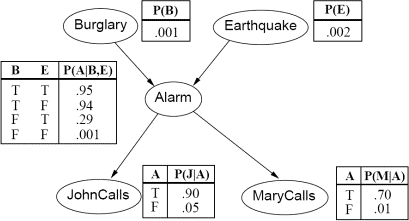
\includegraphics{burglary.png} \end{center}

\noindent Let's define this Bayesian network.

\begin{small}
\begin{verbatim}
>>> assume('burglary', bernoulli(0.001))
>>> assume('earthquake', bernoulli(0.002))
>>> assume('alarm', ifelse('burglary', ifelse('earthquake', bernoulli(0.95), bernoulli(0.94)), \
...                                    ifelse('earthquake', bernoulli(0.29), bernoulli(0.001))))
>>> assume('johnCalls', ifelse('alarm',  bernoulli(0.9), bernoulli(0.05)))
>>> assume('maryCalls', ifelse('alarm',  bernoulli(0.7), bernoulli(0.01)))
\end{verbatim}
\end{small}

\noindent Let's try a couple inference problems.

\begin{small}
\begin{verbatim}
>>> follow_prior('alarm', 1000, 100) # should give 0.002516 True
{False: 0.99739999999999995, True: 0.0025999999999999999}
>>>
>>> noise_level = .001
>>> mary_ob = observe(bernoulli_noise('maryCalls', noise_level), True)
>>> follow_prior('johnCalls', 1000, 100) # should give 0.177577 True
{False: 0.91620000000000001, True: 0.083799999999999999}
>>>
>>> forget(mary_ob)
>>> burglary_ob = observe(bernoulli_noise(negation('burglary'), noise_level), True)
>>> follow_prior('johnCalls', 1000, 100) # should give 0.051343 True
{False: 0.94710000000000005, True: 0.052900000000000003}
\end{verbatim}
\end{small}

The first and third inferences were on the mark, but the second one was off by a factor of two!   The explanation is that Mary calls very rarely calls.  Indeed, she only calls about 0.01 of the time, since the alarm almost never sounds.  This is rare enough that our observation that she called is reasonably likely to be wrong.  In worlds where she doesn't call, John also tends not to call, thus accounting for the large dip. \vspace{6 pt}

To verify that this is the explanation, we can alter the probabilities so that Mary calling is more likely.  Here is an example of this being done.

\begin{small}
\begin{verbatim}
>>> reset()
>>>
>>> assume('burglary', bernoulli(0.1))
>>> assume('earthquake', bernoulli(0.2))
>>> assume('alarm', ifelse('burglary', ifelse('earthquake', bernoulli(0.95), bernoulli(0.94)), \
...                                    ifelse('earthquake', bernoulli(0.29), bernoulli(0.10))))
>>> assume('johnCalls', ifelse('alarm',  bernoulli(0.9), bernoulli(0.5)))
>>> assume('maryCalls', ifelse('alarm',  bernoulli(0.7), bernoulli(0.1)))
>>>
>>> follow_prior('alarm', 1000, 100) # should give 0.218400 True
{False: 0.77959999999999996, True: 0.22040000000000001}
>>>
>>> noise_level = .001
>>> mary_ob = observe(bernoulli_noise('maryCalls', noise_level), True)
>>> follow_prior('johnCalls', 1000, 100) # should give 0.764681 True
{False: 0.2432, True: 0.75680000000000003}
>>>
>>> forget(mary_ob)
>>> burglary_ob = observe(bernoulli_noise(negation('burglary'), noise_level), True)
>>> follow_prior('johnCalls', 1000, 100) # should give 0.561333 True
{False: 0.44290000000000002, True: 0.55710000000000004}
\end{verbatim}
\end{small}

\noindent Success!


\subsection{Testing xor}

\noindent Consider the following program, where we simply draw two booleans {\tt a} and {\tt b}, and observe that their xor is {\tt True}:

\begin{small}
\begin{verbatim}
>>> p, q = 0.6, 0.4
>>> noise_level = .01
>>>
>>> assume('a', bernoulli(p))
>>> assume('b', bernoulli(q))
>>> assume('c', var('a') ^ var('b'))
>>>
>>> follow_prior('a', 10000, 100) # should be 0.60 True
{False: 0.3977, True: 0.60229999999999995}
>>>
>>> xor_ob = observe(bernoulli_noise('c', noise_level), True)
>>> follow_prior('a', 10000, 100) # should be 0.69 True
{False: 0.3342, True: 0.66579999999999995}
\end{verbatim}
\end{small}



This second inference is significantly off, and it's not the case that our observation is particularly unlikely.  Here, the burn-in was not enough.  Notice that in order to mix, the program must walk over states which contradict the observed values.  

Suppose we are in the state {\tt \{a:True, b:True\}}.  Then, the random walk is highly discouraged from entering either of the two adjacent states {\tt \{a:True, b:False\}} and {\tt \{a:False, b:True\}}, since worlds in which {\tt a$\oplus$b} is {\tt False} are weighted against, by a factor of 100.  

Let's estimate the amount of burn-in it should take for this random walk to mix.  Suppose we are in a state where {\tt a$\oplus$b} is {\tt True}.  About half the time, we will attempt to enter one of the two adjacent states (the other half of the time, we will keep the same value for that flip).  Entering this state will occur with probability roughly $\frac{1}{100}$.  Once we are in such a state, we are given an opportunity to enter either of the two {\tt a$\oplus$b} being {\tt True} states, so we have successfully mixed.  

Thus we can roughly model this as having a $\frac{1}{200}$ chance of mixing properly, for each iteration.  Thus if we have a burn-in of $200 \cdot x$, there is roughly a $1 - \frac{1}{e^x}$ chance of mixing.  Here are empirical results of {\tt burnin} against {\tt follow\_prior('a', 10000, burnin)} results:

\begin{center}
\begin{tabular}{|c | c|} \hline
{\tt burnin} & {\tt follow\_prior('a', 10000, burnin)} percentage {\tt True}  \\ \hline
100 &  0.66579999999999995 \\ \hline
200 &  0.67869999999999997 \\ \hline
300 &  0.68200000000000005 \\ \hline
400 &  0.68489999999999995 \\ \hline
500 &  0.68759999999999999 \\ \hline
\end{tabular}
\end{center}

These results are slightly better than our prediction, but confirm the overall phenomenon.  Because of the noise, we can't expect it to ever converge to exactly 0.69.  Instead, we may hope for it to converge to something like $0.01 \cdot 0.60 + 0.99 \cdot 0.69 = 0.6891$.  


\subsection{Testing a decaying atom}

Suppose we are observing a radioactive atom in discrete time intervals, e.g. we look at it each second.  Each time we look at the atom, there is some chance $p$ that it decays, called its decay rate.  

Suppose there is an atom whose decay rate we don't know.  So our prior over decay rates is uniform.  

\begin{small}
\begin{verbatim}
>>> assume('decay', beta(1, 1)) 
>>> assume('geometric', function('x', ifelse(bernoulli('decay'), 'x', apply('geometric', var('x') + 1))))
>>> observe(bernoulli_noise(apply('geometric', 0) == 10, .01), True)
  print get_pdf(follow_prior('decay', 100, 100), 0, 1, .1) 

\end{verbatim}
\end{small}

\subsection{Testing mem}

Here, we test that the memoization procedure works.  

\noindent Let's first write the fibonacci function, in the naive way:

\begin{small}
\begin{verbatim}
>>> fibonacci_expr = function('x', ifelse(var('x')<=1, 1, \
...                  apply('fibonacci', var('x')-1) + apply('fibonacci', var('x')-2)))
>>> assume('fibonacci', fibonacci_expr)
\end{verbatim}
\end{small}

\noindent Of course, evaluating fibonacci in this manner is an exponential time operation:

\begin{small}
\begin{verbatim}
>>> t = time(); sample(apply('fibonacci', 20)); time() - t
10946
1.76103687286
\end{verbatim}
\end{small}

\noindent Mem is an XRP which, when applied to (possibly probabilistic) functions, returns a version of the function which is memoized.  That is, function calls are remembered, so that if a function is called with the same arguments, it does not need to recompute.  Here is an example of mem being used.

\begin{small}
\begin{verbatim}
>>> assume('bad_mem_fibonacci', mem('fibonacci'))
>>>
>>> t = time(); sample(apply('bad_mem_fibonacci', 20)); time() - t
10946
1.90201187134
>>> t = time(); sample(apply('bad_mem_fibonacci', 20)); time() - t
10946
0.00019097328186
\end{verbatim}
\end{small}

\noindent Notice that the second call to this mem'd fibonacci is much faster, since mem remembers the value.  However, the first call is just as slow as before.  Since Fibonacci is recursive, we really want to memoize all the recursive subcalls as well.  The canonical introduction to dynamic programming shows how Fibonacci can be computed in linear time this way.  We can write the program easily:

\begin{small}
\begin{verbatim}
>>> mem_fibonacci_expr = function('x', ifelse(var('x')<=1, 1, \
...                    apply('mem_fibonacci', var('x')-1) + apply('mem_fibonacci', var('x')-2)))
>>> assume('mem_fibonacci', mem(mem_fibonacci_expr))
>>>
>>> t = time(); sample(apply('mem_fibonacci', 20)); time() - t
10946
0.0271570682526
>>> t = time(); sample(apply('mem_fibonacci', 20)); time() - t
10946
0.000293016433716
\end{verbatim}
\end{small}

\subsection{Testing DPMem}

Let's now implement the Dirichlet process.  

\begin{small}
\begin{verbatim}
>>> sticks_expr = mem(function('j', beta(1, 'concentration2')))
>>> atoms_expr = mem(function('j', apply('basemeasure2')))
>>> loop_body_expr = function('j', ifelse(bernoulli(apply('sticks', 'j')), apply('atoms', 'j'), \
...                  apply(apply('loophelper', ['concentration2', 'basemeasure2']), var('j')+1)))
>>> loop_expr = apply(function(['sticks', 'atoms'], loop_body_expr), [sticks_expr , atoms_expr])
>>> assume('loophelper', function(['concentration2', 'basemeasure2'], loop_expr))
>>> assume( 'DP', function(['concentration', 'basemeasure'], \
...                        apply(apply('loophelper', ['concentration', 'basemeasure']), 1)))
\end{verbatim}
\end{small}

We can now use the Dirichlet process to create something we call DPmem.  DPmem is a generalization of mem which sometimes returns memoized values, and sometimes resamples new values.  

\begin{small}
\begin{verbatim}
  """DEFINITION OF DPMEM"""
  restaurants_expr = mem(function('args', apply('DP', ['alpha', function([], apply('proc', 'args'))])))
  assume('DPmem', function(['alpha', 'proc'], function('args', apply(restaurants_expr, 'args'))))


  """TESTING DPMEM"""

  concentration = 1 # when close to 0, just mem.  when close to infinity, sample 
  assume('DPmemflip', apply('DPmem', [concentration, function(['x'], bernoulli(0.5))]))
  print [sample(apply('DPmemflip', 5)) for i in xrange(10)]

  print "\n TESTING GAUSSIAN MIXTURE MODEL\n"
  assume('concentration', gaussian(1, 0.2)) # use vague-gamma? 
  assume('expected-mean', gaussian(0, 1)) 
  assume('expected-variance', gaussian(0, 1))
  assume('gen-cluster-mean', gaussian(0, 1))
  assume('get-datapoint', mem( function(['id'], gaussian('gen-cluster-mean', 1.0))))
  assume('outer-noise', gaussian(1, 0.2)) # use vague-gamma?

  observe(gaussian(apply('get-datapoint', 0), 'outer-noise'), 1.3)
  observe(gaussian(apply('get-datapoint', 0), 'outer-noise'), 1.2)

  t = time()
  print format(get_pdf(follow_prior('expected-mean', 100, 30), -4, 4, .5), '%0.2f')
  print 'time taken', time() - t

  #concentration = 1
  #uniform_base_measure = uniform_no_args_XRP(2)
  #print [sample(apply('DP', [concentration, uniform_base_measure])) for i in xrange(10)]
  #expr = beta_bernoulli_1()

\end{verbatim}
\end{small}


DPmem can be used, for example, to do mixture modeling.  The idea is that we should sometimes


\pagebreak

\begin{thebibliography}{99}

%\bibitem[1]{Fagin1} Fagin, R.  {\em Generalized first-order spectra and polynomial-time recognizable sets}. Complexity of Computation, ed. R. Karp, SIAM-AMS Proceedings 7, 1974, pp. 43--73. 


\end{thebibliography}

\end{document}

